% Version 2: Theme, Logo, Boxes
\documentclass[11pt]{beamer}

%\usetheme{Marburg}
\usetheme{Madrid}
\setbeamertemplate{navigation symbols}{}
\logo{
\includegraphics[height=0.5cm]{ssn-logo.jpg}}

\title{Presentation in \LaTeX}
\author[Milton]{R~S~Milton}
\institute[]{
  Department of Computer Science\\
  SSN College of Engineering
}

\date[]{18 February 2016}

\begin{document}

\begin{frame}
  \titlepage
\end{frame}

\begin{frame}{Outline of the talk}
  \tableofcontents
\end{frame}


\section{Quick presentation}

\begin{frame}{Simple presentation}
  With LaTeX Beamer, we can make consistently looking
  presentation.
  \begin{itemize}
  \item Use \texttt{beamer} class.
  \item Choose a theme.
  \item Otherwise, usual \LaTeX.
  \end{itemize}
\end{frame}

\begin{frame}
  \frametitle{Simplicity}
  Use simple and direct words.
  \begin{block}{Herman Melville}
    A man of true science \ldots uses but few hard words, and
    those only when none other will answer his purpose; whereas
    the smatterer in science\ldots thinks, that by mouthing
    hard words, he proves that he understands hard things.
  \end{block}
  \begin{alertblock}{Herman Melville}
    A man of true science \ldots uses but few hard words, and
    those only when none other will answer his purpose.
  \end{alertblock}
  \begin{exampleblock}
    {Herman Melville}
    A man of true science \ldots uses but few hard words, and
    those only when none other will answer his purpose.
  \end{exampleblock}
\end{frame}

\begin{frame}
  \frametitle{Simplicity}
  Use simple and direct words.
  \begin{columns}
    \begin{column}{.45\textwidth}
      \begin{block}{Herman Melville}
        A man of true science \ldots uses but few hard words,
        and those only when none other will answer his purpose;
        whereas the smatterer in science\ldots thinks, that by
        mouthing hard words, he proves that he understands hard
        things.
      \end{block}
    \end{column}
    \begin{column}{.45\textwidth}
        A man of true science \ldots uses but few hard words,
        and those only when none other will answer his purpose;
        whereas the smatterer in science\ldots thinks, that by
        mouthing hard words, he proves that he understands hard
        things.
    \end{column}
  \end{columns}
\end{frame}

\begin{frame}
  \frametitle{What is Computer Science?}
  \begin{columns}
    \begin{column}{.5\textwidth}
    \begin{center}
      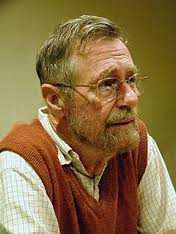
\includegraphics[scale=.5]{dijkstra.jpeg}
    \end{center}      
    \end{column}
    \begin{column}{.5\textwidth}
      \begin{exampleblock}{}
        Computer Science is no more about computers than
        astronomy is about telescopes or biology is about
        microscopes (E W Dijkstra).
      \end{exampleblock}
    \end{column}
  \end{columns}
\end{frame}

\section{Questions}
\begin{frame}{}
  \vfill
  \begin{center}
    Questions?
  \end{center}
  \vfill
  
\end{frame}
\end{document}
